\documentclass [hyperref={bookmarksdepth=4}, aspectratio=169] {beamer}
\usetheme {Berlin}
\def \mathfamilydefault {\rmdefault}
\usepackage {xeCJK}
\usepackage {latexsym, amsmath, amssymb, amsfonts, amstext}
\usepackage {amsbsy, amsopn, xcolor, ulem, listings, tikz, multirow, multicol}

\setCJKmainfont [ItalicFont=KaiTi, BoldFont=SimHei] {SimSun}
\parindent2em

\newfontfamily \codefont {Consolas}

\defbeamertemplate*{headline}{miniframes double theme}{
\begin{beamercolorbox}[colsep=1.5pt]{upper separation line head}\end{beamercolorbox}
\begin{beamercolorbox}{section in head/foot}\vskip2pt\insertnavigation\paperwidth\vskip2pt\end{beamercolorbox}
\begin{beamercolorbox}[colsep=1.5pt]{middle separation line head}\end{beamercolorbox}
\begin{beamercolorbox}[ht=2.5ex,dp=1.125ex,leftskip=.3cm,rightskip=.3cm plus1fil]{subsection in head/foot}\leavevmode{\usebeamerfont{subsection in head/foot}\insertsubsectionhead}\hfill{\usebeamerfont{subsubsection in head/foot}\insertsubsubsectionhead}\end{beamercolorbox}
\begin{beamercolorbox}[colsep=1.5pt]{lower separation line head}\end{beamercolorbox}
}
\setbeamertemplate {theorems} [numbered]
\setbeamertemplate {headline} [miniframes double theme]
\setbeamertemplate {navigation symbols} {}

\newtheoremstyle {fy} {6pt} {6pt} {\it} {25pt} {\bfseries} {.} {4pt} {}
\theoremstyle {fy}
\newtheorem {rawtheo} {Theorem} [subsection]
\newenvironment {theo} [1] [] {\begin{rawtheo} [#1] \parindent2em} {\end{rawtheo}}
\def \rawtheoautorefname {Theorem}
\newtheorem {rawdefi} {Definition} [subsection]
\newenvironment {defi} [1] [] {\begin{rawdefi} [#1] \parindent2em} {\end{rawdefi}}
\newtheorem {rawcoro} {Corollary} [subsection]
\newenvironment {coro} [1] [] {\begin{rawcoro} [#1] \parindent2em} {\end{rawcoro}}
\def \rawcoroautorefname {Corollary}
\newtheorem {raweg} {Example}
\newenvironment {eg} [1] [] {\begin{raweg} [#1] \parindent2em} {\end{raweg}}
\newtheorem*{rawsolu} {Solution}
\newenvironment {solu} [1] [] {\begin{rawsolu} [#1] \parindent2em} {\end{rawsolu}}

\usetikzlibrary {positioning}
\tikzset {every picture/.style={inner sep=-6pt}, vertices/.style={every node/.style={circle, draw, minimum size=16pt}}, block vertex/.style={rectangle, draw, minimum size=12pt, rounded corners=2.5pt}}
\definecolor {cgreen} {rgb} {0, .75, 0}

\lstset {
	backgroundcolor=\color{white},
	basicstyle=\text\tt\scriptsize\codefont,
	columns=fullflexible,
	tabsize=4,
	breaklines=true,
	captionpos=b,
	escapeinside={(@}{@)},
	commentstyle=\color{teal},
	keywordstyle=\color{blue},
	numbers=left,
	numberstyle=\color{magenta},
	stringstyle=\color{purple},
	frame=single,
	language=c++,
}

% 补充 Markdown 中使用的数学符号定义
\def\Z{\mathbb{Z}}
\def\R{\mathbb{R}}
\def\Q{\mathbb{Q}}
\def\C{\mathbb{C}}
\def\N{\mathbb{N}}
\def\P{\mathbb{P}}

% 在每个 Section 前自动插入展示该模块内部结构的目录
% \AtBeginSection[]{
%   \begin{frame}[allowframebreaks]{本章目录}
%     \begin{multicols}{2}
%       \tableofcontents[currentsection, hideothersubsections]
%     \end{multicols}
%   \end{frame}
% }

\AtBeginSubsection[]{
  \begin{frame}{本节导航}
    \begin{multicols}{2}
      \tableofcontents[
        sectionstyle=show/shaded,         % 当前大章显色，其他大章淡化
        subsectionstyle=show/shaded/hide, % 精准控制：当前小节高亮 / 同章其他淡化 / 其他大章的小节隐藏
        subsubsectionstyle=hide           % 隐藏所有更小的子小节
      ]
    \end{multicols}
  \end{frame}
}


\begin {document}

\title {数论}
\author {}
\date {}

\frame \titlepage

\subsection*{目录}

\begin{frame}[fragile,allowframebreaks]{目录}
	\begin{multicols}{3}
		\tableofcontents[subsubsectionstyle=hide]
	\end{multicols}
\end{frame}

\section{整除}

\subsection{整除理论}

\subsubsection{基本定义}

\begin{frame}[fragile,allowframebreaks]{}
我们知道任意两个整数的和、差、积以至任意有限个整数的加、减、乘的混合运算结果仍是整数，但是整数除整数不一定仍为整数。

为了应对整数除法的不封闭性，我们引入整除的概念。

\begin{itemize}
    \item 整除的定义

  设 $a,b$ 是任意两个整数，其中 $b\neq 0$，若存在整数 $q$ 使得 $a=bq$，则称 $b$ 整除 $a$ 或 $a$ 被 $b$ 整除，记作 $b\mid a$。
\end{itemize}

此时称 $b$ 为 $a$ 的因数，$a$ 为 $b$ 的倍数。

\begin{itemize}
    \item 重要性质

  $d\mid a,d\mid b\implies d\mid ua+vb\ (u,v\in\Z)$

    \item 带余除法的定义

  设 $a,b$ 是任意两个整数，其中 $b\neq 0$，存在唯一的整数对 $(q,r)$ 使得 $a=bq+r$ 且 $0\le r<|b|$。记作 $a\div b=q\cdots r$。
\end{itemize}

此时称 $q$ 为 $a$ 除以 $b$ 的商，$r$ 为 $a$ 除以 $b$ 的余数。记 $a\bmod b=r$。
\end{frame}

\begin{frame}[fragile,allowframebreaks]{取整函数}
对于任意 $x\in \R$，用 $\left[x\right]$ 或 $\lfloor x \rfloor$ 表示不大于 $x$ 的最大整数。用 $\lceil x\rceil$ 表示不小于 $x$ 的最小整数。用 $\left\{x\right\}=x-\lfloor x\rfloor$ 表示 $x$ 的小数部分。

（$\left[x\right]$ 由高斯提出，是 19 世纪初等数论的产物。$\lfloor x \rfloor$ 由计算机科学大师高德纳于 1962 年提出，更加适配计算机科学的语境与应用场景。建议大家以后一律使用 $\lfloor x\rfloor$）

\begin{itemize}
    \item 简单性质

  $\lfloor x\rfloor\le x<\lfloor x\rfloor+1$，$x-1<\lfloor x\rfloor\le x$

  $\lfloor n+x\rfloor=n+\lfloor x\rfloor$，$n$ 为整数

  $\lfloor x\rfloor+\lfloor y\rfloor\le\lfloor x+y\rfloor$

  $a,b\in\Z,b>0$，则 $a=b\left\lfloor\dfrac{a}{b}\right\rfloor+b\left\{\dfrac{a}{b}\right\}$

    \item 复合性质

  $m\in\Z^{+},x\in\R$，则 $\left\lfloor\dfrac{x}{m}\right\rfloor=\left\lfloor\dfrac{\lfloor x\rfloor}{m}\right\rfloor$

  $a\in\Z,b,c\in\Z^{+}$，则 $\left\lfloor\dfrac{a}{bc}\right\rfloor=\left\lfloor\dfrac{\left\lfloor\frac{a}{b}\right\rfloor}{c}\right\rfloor$
\end{itemize}
\end{frame}

\subsection{最大公因数}

\begin{frame}[fragile,allowframebreaks]{基本定义}
\begin{itemize}
    \item gcd \& lcm

  $a,b\in \Z$，若 $d\mid a,d\mid b$，则称 $d$ 为 $a,b$ 的公因数。

  当 $a,b$ 不全为 $0$ 时公因数个数是有限的，故存在最大公因数，记为 $\gcd(a,b)$ 或 $(a,b)$。

  特别地，若 $a=b=0$，定义 $\gcd(0,0)=0$。

  同理定义最小公倍数，记为 $\mathrm{lcm}(a,b)$ 或 $\left[a,b\right]$。
\end{itemize}
\end{frame}

\begin{frame}[fragile,allowframebreaks]{基本性质}
\begin{itemize}
    \item 基本性质

  $\gcd(a,b)=\gcd(|a|,|b|)$

  $\gcd(\gcd(a,b),c)=\gcd(a,\gcd(b,c))$

  $\mathrm{lcm}(\mathrm{lcm}(a,b),c)=\mathrm{lcm}(a,\mathrm{lcm}(b,c))$

  （如果把 $\gcd$ 或 $\mathrm{lcm}$ 看做一个二元运算 $\oplus$，这意味着 $a_1\oplus\dots\oplus a_n$ 可以任意加括号）

  （在表达式树上这种操作意味着左旋和右旋，一棵树一定可以通过右旋变成一棵标准的右斜链，然后再通过左旋变成任意形状的树）

  $\gcd(a,b)\mathrm{lcm}(a,b)=ab$

  $d\mid a,d\mid b\iff d\mid\gcd(a,b)$

  $\gcd(ma,mb)=m\gcd(a,b)$

  $\gcd(a^n,b^n)=\gcd(a,b)^n$
\end{itemize}
\end{frame}

\begin{frame}[fragile,allowframebreaks]{欧几里得算法}
$\gcd$ 有以下性质：

$\gcd(a,b)=\gcd(b,a-b)$

$\gcd(a,b)=\gcd(b,a\bmod b)$

由此得到求 $\gcd$ 的欧几里得算法：

\begin{lstlisting}
int gcd(int a, int b) {
    if (b == 0) return a;
    return gcd(b, a % b);
}
\end{lstlisting}

每次操作后 $ab$ 至少会变为原来的 $1/2$，故时间复杂度 $O(\log a+\log b)$。

精细的分析是 $O(\log\min\{a,b\})$。

更加精细的分析是递归次数不超过 $\log_{\phi}\dfrac{\min\{a,b\}}{\gcd(a,b)}+O(1)$。其中 $\phi=\dfrac{1+\sqrt{5}}{2}$。
\end{frame}

\begin{frame}[fragile,allowframebreaks]{例题}
求 $\gcd(2^{120}-1,2^{100}-1)$。
$$
\begin{aligned}
\gcd(a^n-1,a^m-1)
=&\gcd(a^n-a^m,a^m-1)\\
=&\gcd(a^m(a^{n-m}-1),a^m-1)\\
=&\gcd(a^{n-m}-1,a^m-1)
\end{aligned}
$$
对指数使用辗转相除法，可证 $\gcd(a^n-1,a^m-1)=a^{\gcd(n,m)}-1$。

可以再思考证明：$\gcd(a,b)=1$，则 $\gcd(a^m-b^m,a^n-b^n)=a^{\gcd(m,n)}-b^{\gcd(m,n)}$。
\end{frame}

\begin{frame}[fragile,allowframebreaks]{裴蜀定理}
\begin{itemize}
    \item 裴蜀定理

  若 $a,b$ 为整数且 $\gcd(a,b)=d$，则 $\forall x,y\in\Z,d\mid ax+by$。且存在一组 $x,y$ 使得 $ax+by=d$。
\end{itemize}

裴蜀定理告诉我们存在这样的 $x,y$。下面的扩展欧几里得算法可以找出一组特定的 $x,y$。

\begin{itemize}
    \item 扩展欧几里得算法
\end{itemize}

\begin{lstlisting}
int exgcd(int a, int b, int &x, int &y) {
    if (b == 0) {
        x = 1; y = 0;
        return a;
    }
    int d = exgcd(b, a % b, y, x);
    y -= a / b * x;
    return d;
}
\end{lstlisting}

利用归纳法，可知求出的 $x,y$ 满足 $|x|\le b,|y|\le a$。
\end{frame}

\begin{frame}[fragile,allowframebreaks]{二元一次不定方程}
对于方程 $ax+by=c$，其有解的充要条件是 $\gcd(a,b)\mid c$。

调用 exgcd，得到的结果记为 $x_0,y_0$。

一组特解为 $x_1=\dfrac{x_0c}{\gcd(a,b)},y_1=\dfrac{y_0c}{\gcd(a,b)}$。

通解为 $x=x_1+k\dfrac{b}{\gcd(a,b)},y=y_1-k\dfrac{a}{\gcd(a,b)}$。其中 $k$ 为任意整数。
\end{frame}

\begin{frame}[fragile,allowframebreaks]{P3518 [POI 2011] SEJ-Strongbox}
有一个密码箱，$0$ 到 $n-1$ 中的某些整数是它的密码。且满足：若 $a$ 和 $b$ 是它的密码，则 $(a+b)\bmod n$ 也是它的密码（$a,b$ 可以相等）。某人试了 $k$ 次密码 $m_1,\dots,m_k$，前 $k-1$ 次都失败了，最后一次成功了。问，该密码箱最多有多少种不同的密码。

$1\le k\le 2.5\times 10^5,k\le n\le 10^{14}$。

设最小非零的密码为 $d$，则所有 $d$ 的倍数也是密码。若存在密码 $x$ 不是 $d$ 的倍数，则由裴蜀定理 $\gcd(x,d)<d$ 也是密码，与 $d$ 的最小性矛盾。故所有密码恰是 $d$ 的所有倍数。进一步可知 $d\mid n$。

故枚举 $\gcd(n,m_k)$ 的所有因子，找到最小的 $d$ 满足 $d\nmid m_i\ (i<k)$ 即为答案。精细实现可将复杂度优化至 $O(d(n)\omega(n))$。
\end{frame}

\section{同余}

\subsection{定义}

\begin{frame}[fragile,allowframebreaks]{同余定义}
好的符号体系可以大大降低描述问题的难度，使得我们能把更多精力放在问题本身上。例如下面是一套不好的符号体系：

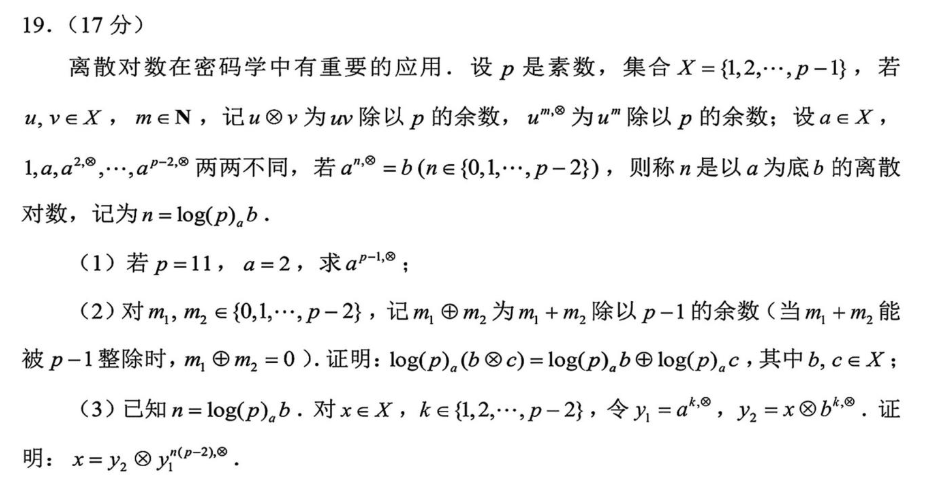
\includegraphics[width=0.7\textwidth]{pic1.png}

\begin{itemize}
    \item 同余定义

  给定一个正整数 $m$，若整数 $a,b$ 除以 $m$ 的余数相同，则称 $a,b$ 关于模 $m$ 同余，记为 $a\equiv b\pmod m$。
\end{itemize}

使用同余的符号体系，可以在处理加、减、乘等运算时像普通的等式一样方便地进行代数变形。

若 $a\equiv b\pmod m,c\equiv d\pmod m$，则 $a+c\equiv b+d\pmod m$，$a-c\equiv b-d\pmod m$，$ac\equiv bd\pmod m$，$a^n\equiv b^n\pmod m$。

若 $ac\equiv bc\pmod m$，且 $\gcd(c,m)=d$，则 $a\equiv b\pmod{\dfrac{m}{d}}$。

（补全乘法逆元的存在性：$\gcd(c,m)=1$ 时，该式就是两边同乘 $c^{-1}$。但 $c^{-1}$ 不存在时，该式相当于取新的模数 $m'=\dfrac{m}{\gcd(c,m)}$，此时 $\gcd(c,m')=1$，故在新的模数下 $c^{-1}$ 存在）
\end{frame}

\begin{frame}[fragile,allowframebreaks]{剩余类和剩余系}
\begin{itemize}
    \item 剩余类

  设 $m$ 是一个正整数，任意整数除以 $m$ 所得的余数有 $m$ 中可能 $0,1,\dots,m-1$。对于一种余数 $r$，所有模 $m$ 与 $r$ 同余的整数形成集合 $[r]=\{km+r\mid k\in\Z\}$，称为模 $m$ 的一个剩余类。

    \item 完全剩余系

  设 $a_0,a_1,\dots,a_{m-1}$ 是 $m$ 个整数，若其中任意两数都不在同一个剩余类中，则称 $\{a_0,a_1,\dots,a_{m-1}\}$  为模 $m$ 的一个完全剩余系，简称完系。
\end{itemize}

特别地，$\{0,1,\dots,m-1\}$ 称为模 $m$ 的最小非负完系。

\begin{itemize}
    \item 欧拉函数

  欧拉函数 $\varphi(a)$ 为定义在正整数上的函数，$\varphi(a)$ 等于 $0,1,\dots,a-1$ 中与 $a$ 互素的数的个数。

    \item 简化剩余系

  设 $a_0,a_1,\dots,a_{\varphi(m)-1}$ 是 $\varphi(m)$ 个整数，若其中任意两数都不在同一剩余类中，且每个数都与 $m$ 互素，则称 $\{a_0,a_1,\dots,a_{\varphi(m)-1}\}$ 为模 $m$ 的一个简化剩余系或既约剩余系，简称缩系。
\end{itemize}

尝试证明一下性质：

\begin{itemize}
    \item 性质

  若 $x$ 取遍模 $m$ 的完全剩余系，则 $ax+b$ 也取遍模 $m$ 的完全剩余系。

  若 $\gcd(a,m)=1$，$x$ 取遍模 $m$ 的简化剩余系，则 $ax$ 也取遍模 $m$ 的简化剩余系。

  若 $x_1,x_2$ 分别取遍模 $m_1,m_2$ 的完全剩余系，则 $m_2x_1+m_1x_2$ 取遍模 $m_1m_2$ 的完全剩余系。

  若 $m_1,m_2$ 互素，$x_1,x_2$ 分别取遍模 $m_1,m_2$ 的简化剩余系，则 $m_2x_1+m_1x_2$ 取遍模 $m_1m_2$ 的简化剩余系。

  推论：$\varphi(m_1m_2)=\varphi(m_1)\varphi(m_2)$。
\end{itemize}
\end{frame}

\subsection{乘法逆元}

\begin{frame}[fragile,allowframebreaks]{逆元}
有些问题在一个数系中难以解决，但通过数系的扩张可以变简单。

\begin{itemize}
    \item 从 $\Z$ 到  $\Q$

  计算 $9396\times 14\div 21$。

  这是一个 $\Z$ 上的问题，完全限制在 $\Z$ 上也能做但是运算复杂。引入 $\Q$ 可以简化运算。

    \item 从 $\R$ 到 $\C$

  求三次方程 $x^3-3x+1=0$。

  看函数图像可知该方程有三个实根。但是完全限制在 $\R$ 上不容易求出，引入 $\C$ 后可以通过求根公式快速求出。中间过程会产生虚数单位 $i$，但最后全部消掉，结果回到 $\R$ 中。

    \item 逆元定义

  设 $m$ 是一个大于 $1$ 的正整数，$a$ 是任意一个整数。若存在整数 $x$ 使得 $ax\equiv 1\pmod m$ 成立，则称 $x$ 为 $a$ 模 $m$ 的乘法逆元，记为 $a^{-1}$。
\end{itemize}

$ax\equiv 1\pmod m\iff ax+m\xi=1$。由裴蜀定理，$a$ 存在逆元的充要条件是 $\gcd(a,m)=1$。

所有逆元属于同一个剩余类。

模为素数 $p$ 时，每个整数 $0<x<p$ 均有逆元。

\begin{itemize}
    \item 例题

  求解线性同余方程 $3x\equiv 4\pmod{101}$。

  原来需要解二元一次方程，现在只需两边同乘 $3$ 的逆元即可。
\end{itemize}

乘法逆元可以在同余的体系下引入人造分数，在运算上和 $\Q$ 保持高度一致。以后可以使用 $\dfrac{a}{b}$ 来表示 $a\cdot b^{-1}\bmod m$。
\end{frame}

\begin{frame}[fragile,allowframebreaks]{逆元求解}
求逆元的第一种方法是使用 exgcd 求二元一次方程，前面已经介绍过。下面介绍 OI 中更常用的利用欧拉定理的方法。

\begin{itemize}
    \item 欧拉定理

  对于大于 $1$ 的正整数 $m$ 和与 $m$ 互素的整数 $a$，有 $a^{\varphi(m)}\equiv 1\pmod m$。

  由前面的结论，当 $x$ 取遍模 $m$ 的简化剩余系时，$ax$ 也取遍模 $m$ 的简化剩余系。设 $\{r_1,r_2,\dots,r_{\varphi(m)}\}$ 是一个简化剩余系，则 $r_1r_2\dots r_{\varphi(m)}\equiv a^{\varphi(m)}r_1r_2\dots r_{\varphi(m)}\pmod m$。又 $\gcd(r_1,m)=\gcd(r_2,m)=\dots=\gcd(r_{\varphi(m)},m)=1$，故 $\gcd(r_1r_2\dots r_{\varphi(m)},m)=1$。于是 $a^{\varphi(m)}\equiv 1\pmod m$。

    \item 费马小定理

  对于素数 $p$ 和模 $p$ 不为 $0$ 的整数 $a$，$a^{p-1}\equiv 1\pmod p$。
\end{itemize}

于是 $a$ 的逆元可以直接表示为 $a^{\varphi(m)-1}$ 或 $a^{p-2}$。

exgcd 和快速幂都需要 $\log$ 时间复杂度，下面介绍一种离线的线性预处理、$O(1)$ 查询的逆元求法。

\begin{itemize}
    \item 离线逆元

  有 $n$ 个整数 $a_1,a_2,\dots,a_n$，用线性时间求出它们在模 $m$ 意义下的逆元 $a_1^{-1},a_2^{-1},\dots,a_n^{-1}$。

  记 $A=a_1a_2\dots a_n$。由于每个 $a_i$ 都有逆元，$A$ 也有逆元 $A^{-1}$。

  维护序列的前缀积 $p_i=a_1a_2\dots a_{i-1}$ 和后缀积 $s_i=a_{i+1}a_{i+2}\dots a_n$。则 $a_i^{-1}\equiv A^{-1}p_{i-1}s_{i+1}\pmod m$。
\end{itemize}

特别地，$1\sim n$ 中所有数的逆元、$1\sim n$ 中所有数的阶乘的逆元也可以线性预处理。
\end{frame}

\begin{frame}[fragile,allowframebreaks]{SOJ123 水题}
给定奇质数 $P$ 和 $n$ 个整数 $a_1,\dots,a_n$，支持两种操作：

1. 对于所有 $l\le i\le r$，将 $a_i$ 加上 $x$。
2. 对于所有 $l\le i\le r$，将 $a_i$ 变成 $a_i^{P-2}$。

每次操作后输出 $\sum\limits_{i=1}^na_i\bmod P$。$n\le 2000$，操作次数 $m\le 2000$。

将每个 $a_i$ 以分数的形式维护，每次查询的时候线性求出每个分母的逆元。复杂度 $O(nm+m\log P)$。
\end{frame}

\end {document}